\documentclass[landscape]{article}
\usepackage[landscape,margin=0.7in]{geometry}
\usepackage{pgfplots}
\usepackage{tikz}
\pgfplotsset{compat=1.18}

\begin{document}
\pagestyle{empty}

\begin{figure}
    \centering
    \begin{tikzpicture}
        \begin{axis}[
            title={\Large Random Strategy - Step 3: Final Boarding Phase (t = 22 minutes)},
            xlabel={Seat Column},
            ylabel={Row Number},
            xticklabels={A,B,C,D,E,F},
            ytick={1,2,3,4,5,6,7,8,9,10,11,12,13,14,15,16,17,18,19},
            xtick={0,1,2,3,4,5},
            xmin=-0.5,
            xmax=5.5,
            ymin=0.5,
            ymax=19.5,
            y dir=reverse,
            enlargelimits=false,
            axis on top,
            width=0.9\textwidth,
            height=0.4\textheight,
            colorbar,
            colormap={boarding}{
                color(0)=(white);
                color(0.5)=(yellow);
                color(1)=(purple)
            },
            colorbar style={
                title={Status},
                ytick={0,0.5,1},
                yticklabels={Empty,Boarding,Seated},
            },
            point meta min=0,
            point meta max=1
        ]
            
        % Seats with almost all filled in random order (a few still boarding)
        \addplot[matrix plot, mesh/cols=6, point meta=explicit] table [meta=C] {
            x y C
            0 1 1
            1 1 1
            2 1 0.5
            3 1 1
            4 1 1
            5 1 1
            0 2 1
            1 2 1
            2 2 1
            3 2 0.5
            4 2 1
            5 2 1
            0 3 1
            1 3 1
            2 3 0.5
            3 3 1
            4 3 1
            5 3 1
            0 4 1
            1 4 1
            2 4 1
            3 4 0.5
            4 4 1
            5 4 1
            0 5 1
            1 5 0.5
            2 5 1
            3 5 1
            4 5 1
            5 5 1
            0 6 1
            1 6 1
            2 6 1
            3 6 0.5
            4 6 1
            5 6 1
            0 7 1
            1 7 1
            2 7 1
            3 7 1
            4 7 1
            5 7 0.5
            0 8 1
            1 8 1
            2 8 0.5
            3 8 1
            4 8 1
            5 8 1
            0 9 1
            1 9 1
            2 9 1
            3 9 1
            4 9 0.5
            5 9 1
            0 10 1
            1 10 1
            2 10 1
            3 10 0.5
            4 10 1
            5 10 1
            0 11 1
            1 11 1
            2 11 1
            3 11 1
            4 11 1
            5 11 1
            0 12 1
            1 12 0.5
            2 12 1
            3 12 1
            4 12 1
            5 12 1
            0 13 1
            1 13 1
            2 13 1
            3 13 1
            4 13 0.5
            5 13 1
            0 14 1
            1 14 1
            2 14 1
            3 14 1
            4 14 1
            5 14 1
            0 15 0.5
            1 15 1
            2 15 1
            3 15 1
            4 15 1
            5 15 1
            0 16 1
            1 16 1
            2 16 1
            3 16 1
            4 16 1
            5 16 0.5
            0 17 1
            1 17 1
            2 17 1
            3 17 1
            4 17 1
            5 17 1
            0 18 1
            1 18 0.5
            2 18 1
            3 18 1
            4 18 1
            5 18 1
            0 19 1
            1 19 1
            2 19 1
            3 19 1
            4 19 1
            5 19 1
        };
        
        % Draw aisle line
        \draw[black, thick, dashed] (axis cs:2.5,0.5) -- (axis cs:2.5,19.5);
        
        % Time indicator
        \node[font=\Large] at (axis cs:2.5,20.5) {t = 22 minutes};
        
        % Legend for random strategy
        \node[draw, align=left, anchor=south west] at (axis cs:-0.5,-2) {
            \textbf{Random Boarding Strategy:}\\
            After 22 minutes, almost all passengers (95\%) have been seated.\\
            The remaining passengers (5\%) are in the final boarding process.\\
            This strategy results in the longest overall boarding time (22 minutes) compared to other methods.\\
            The inefficiency is due to frequent interferences when passengers need to stand up for others to access their seats.
        };
        \end{axis}
    \end{tikzpicture}
\end{figure}

\end{document}